\section{Theory and Hypothesis}
\label{section:theory_and_hypothesis}


\subsection{PWM Signals}
One of the major theoretical components of this experiment is the Pulse Width Modulation (PWM) signal which, when applied across a load, generates a corresponding RMS voltage. The PWM has a set period, which needs to be faster than the time constant of the circuit, in order to allow the capacitor to retain some charge between successive pulses. Otherwise, the capacitor would discharge completely between each and every PWM cycle, which would cause the overall RMS voltage not to reach the desired value reliably.



The time constant of our RC circuit, with our resistor and capacitor having values of $4.7k\Omega$ and $0.1\mu F$ respectively, was calculated to be approximately 0.47ms, using Equation~\ref{equation:time_constant}. 
\begin{equation}
\tau = RC = 0.1{\mu}F * 4.7k\Omega = 0.47 ms
\label{equation:time_constant}
\end{equation}



The duty cycle of a PWM signal represents the fraction of the period during which the output signal is high. By setting the duty cycle to 0, there would be no active portion in the cycle, which would yield a calculated RMS value of 0 volts. By progressively incrementing the duty cycle, we can expect to start to measure an increasing RMS voltage across the capacitor, as it begins to receive periodic packets of charge during the active duty cycle of our PWM pulse, and then dissipates its charge during the rest of the PWM cycle. By choosing an appropriate value for the duty cycle, we can create an equilibrium where the capacitor gains as much charge during the voltage pulse as it dissipates during the rest of the cycle\footnote{\href{https://en.wikipedia.org/wiki/Pulse-width_modulation}{Pulse-width modulation: Wikipedia}}, effectively maintaining an average voltage over time. Figure \ref{fig:general_pwm_operation} shows an example of such an equilibrium. 


\newcommand*{\captionsource}[2]{%
  \caption[{#1}]{%
    #1%
    \\\hspace{\linewidth}%
    \textbf{Source:} #2%
  }%
}



\begin{figure}[h]
\centering
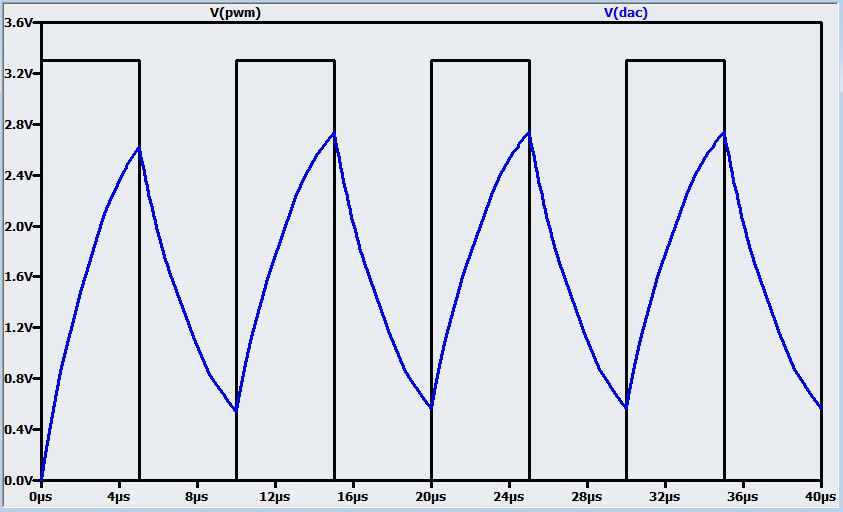
\includegraphics[scale=0.4]{images/PWMDAC2_plot7.jpg}
%
\captionsource{\label{fig:general_pwm_operation}The general shape of a PWM signal in charging/discharging a RC circuit.}{\href{https://www.allaboutcircuits.com/uploads/articles/PWMDAC2_plot7.jpg}{https://www.allaboutcircuits.com}}

\end{figure}

\subsection{Making a PWM Controller}

With our PWM timer created, we need a controller to compare our measured RMS with the target RMS value given by the user via keypad. This controller would then see if the duty cycle needed to be increased, decreased, or kept at the same value, based on if the measured RMS value was above, bellow, or less than \verb|THRESHOLD| away from our target. The implementation of this controller could be quite simple. as it just needs to compare two values in order to determine which action to perform. Here is some pseudocode for such a controller.

\begin{lstlisting}[language=C, basicstyle=\small]

if(ABS(current_RMS - target_RMS) <= THRESHOLD){
	//Don't change anything. We reached the target voltage.
}else if(current_RMS < target_RMS){
	//increase Duty Cycle
}else{
	//decrease Duty Cycle
}
\end{lstlisting}

\subsection{Choosing the PWM and ADC frequencies}

With our time constant of 0.470 ms calculated in Equation~\ref{equation:time_constant}, it is required that the PWM timer period be smaller than this value. Hence, our prediction is that by using a 0.1ms period for our PWM timer, we should be able to successfully generate the required RMS voltage across the capacitor.

Given the corresponding PWM timer frequency of 10KHz, it is important to choose an appropriate value of ADC sampling frequency in order to ensure that we can detect the changes applied by our controller, as well as reliably measure an "average" voltage on the circuit over time, in the form of the RMS of a number of samples. In order to do so, our ADC sampling period needs to be much longer than our PWM signal period, such that the ADC samples are somewhat "randomly" distributed along the capacitor voltage curve (an example of which can be seen in Figure \ref{fig:general_pwm_operation} above). With multiple random samples taken across multiple cycles, our converted ADC values will give an accurate combined RMS voltage value. To that end, we concluded that using the same ADC sampling frequency of 1kHz as in Lab 2 would probably yield positive results.

Following equation \ref{equation:timer_frequency}, the \verb|prescaler| and \verb|period| settings of the ADC will be picked to meet the above requirements and generate a 1 kHz sampling frequency. 

\begin{equation}
\label{equation:timer_frequency}
 Timer freq. = \frac{Clock freq.}{(prescaler + 1) * period}
\end{equation}
%With a \verb|prescaler| of 83, \verb|period| of 1000 and the the Timer frequency of the ADC comes out to be $1kHz$ which falls within our system constraints.


\subsection{Multithreading}



Another requirement of this lab is to implement threads into our system. We did this using the FreeRTOS (Free Real Time Operating System) kernel. This makes available a middleware that is able to schedule and handle the creations of threads and free up the CPU. The advantages of running multiple threads concurrently means that our display thread (which takes care of refreshing our display with the appropriate user input value or measured RMS value of our circuit) and our keypad thread can share CPU time, but exist as separate entities, each with their corresponding logic and program space. Another advantage of running threads in our system is that we are no longer dependent on the internal SysTick Interrupt Handler as a provider of time. 
The ADC can also be modeled as a thread which waits until a \verb|buffer_full| flag indicating that the DMA buffer was filled is set, then compute the RMS value, and go back to sleep. Whether to implement this in a thread or ISR would be logically equivalent, since either these operations are always in the same sequence. The choice of paradigm does make a difference though, as will be explained in the \nameref{section:testing_and_observations} section.

 